\documentclass{mproj}

\usepackage{amsmath}
\usepackage{breakurl}
\usepackage{calc} % for \widthof
\usepackage{pifont} % \for \ding
\usepackage{etoolbox}
\usepackage{float}
\usepackage{listings}
\usepackage{microtype}
\usepackage{url}
\usepackage{xcolor}
\usepackage[T1]{fontenc}
\usepackage[scaled=0.75]{beramono}
\usepackage{graphicx}
\usepackage{xspace}

\usepackage{xspace}
\usepackage{ifthen}

\newif\ifdraft
 \drafttrue

%%%%%%%%%%%%%%%%%%%%%%%%%%%%%%%%%%%%%%%%%%%
% Maths
%%%%%%%%%%%%%%%%%%%%%%%%%%%%%%%%%%%%%%%%%%%

%BNF
\newcommand\DEF{\ \ ::=\ \ }
\newcommand\OR{\ \ |\ \ }

\newcommand{\set}[1]{\{#1\}}
\newcommand{\setbar}{\ \ |\ \ }

\newcommand{\bnfis}{\ensuremath{\ \ ::=\ \ }}
\newcommand{\bnfbar}{\ensuremath{\ \ |\ \ }}


%\def\infrulestyle{\displaystyle}
%\def\infrulestyle{\textstyle}
%\def\makeinfrulesmall{\def\infrulestyle{\textstyle}}
%\def\makeinfrulenormal{\def\infrulestyle{\displaystyle}}
\newcommand{\tree}[4][] {
	\begin{array}{l}
		\ifthenelse { \equal {#1} {} }
		{}
		{
		#1
		\\
		}
		{\textstyle \frac{
			\begin{array}{c}
			#2
			\end{array}
		}{
			\begin{array}{l}
			#3
			\end{array}
		}
		}
		\ifthenelse { \equal {#4} {} }
		{}
		{
		\ #4
		}
	\end{array}
}
\newcommand{\treeline}{\\[6mm]}
\newcommand\andalso{\quad}

%\newcommand{\implies}{\Rightarrow}


%%%%%%%%%%%%%%%%%%%%%%%%%%%%%%%%%%%%%%%%%%%
% Processes
%%%%%%%%%%%%%%%%%%%%%%%%%%%%%%%%%%%%%%%%%%%


\newcommand{\sep}{.}

\newcommand\recover{\,\triangleright\,}
\newcommand\aggr[1]{\breve{#1}}
\newcommand\pout[2]{#1{}!\langle #2\rangle.}
\newcommand\pin[2]{{#1}{}?(#2).}
\newcommand\pll{\,|\,}
\newcommand{\Sum}{\ensuremath{+}\xspace}
\newcommand\sel[2]{#1\triangleleft #2.}
\newcommand\branchOn[2]{#1\,{\triangleright}\,#2}
\newcommand\branch[2]{#1\,{\triangleright}\,\{#2\}}
\newcommand\branchI[3]{\branch{#1}{{#2}_i: {#3}_i}_{i\in I}}
\newcommand{\ndet}[2]{#1 \Sum #2}
\newcommand\rec[1]{\mu #1.}
\newcommand\recvar[1]{X}
\newcommand{\Def}[2]{\ensuremath{\mathsf{def}\ #1\ \mathsf{in}\ #2} \xspace}
\newcommand{\appl}[2]{#1\langle#2\rangle}
\newcommand{\abs}[2]{#1(#2)}

\newcommand{\If}{\ensuremath{\mathsf{if}}\xspace}
\newcommand{\Then}{\ensuremath{\mathsf{then}}\xspace}
\newcommand{\Else}{\ensuremath{\mathsf{else}}\xspace}
\newcommand\cond[3]{\If\,#1\,\Then\,#2\,\Else\,#3}
\newcommand\request[2]{#1!(#2).}
\newcommand\accept[2]{#1?(#2).}
\newcommand\nil{\mathbf{0}}
\newcommand{\un}{\ensuremath{\mathsf{un}}\xspace}
\newcommand{\lin}{\ensuremath{\mathsf{lin}}\xspace}





% \newcommand{\bool}{\ensuremath{\mathsf{bool}}\xspace}
\newcommand{\true}{\ensuremath{\mathsf{true}}\xspace}
\newcommand{\false}{\ensuremath{\mathsf{false}}\xspace}


\newcommand{\newn}[1]{(\nu\,#1)}
\newcommand{\newnp}[2]{\newn{#1}(#2)}

\newcommand{\net}[1]{[#1]}
\newcommand{\npll}{|}
\let\node\net
\newcommand{\assert}{\psi}
\newcommand{\netnil}{\node{\nil\recover\nil}{l}}

\newcommand\condtrue{\Vdash}

% Exprs and conditions
\newcommand{\econd}{\ensuremath{\varphi}\xspace}


%\newcommand\loc[1]{[#1]}
\newcommand\locl[1]{\net{#1}{l}}

\newcommand{\Par}[3]{\prod_{#1 \in #2} #3}

% \newcommand{\cnt}[2]{|#2|_{#1}}
%\newcommand{\cnt}[2]{\mathsf{cnt}(#1, #2)}
\newcommand{\cnt}[1]{\mathsf{cnt}(#1)}
\newcommand{\dom}[1]{\mathrm{dom}(#1)}
\newcommand{\U}[1]{\mathcal{U}(#1)}
\newcommand{\Linset}[1]{\mathcal{L}(#1)}


\newcommand{\mult}{\ensuremath{\odot}\xspace}
\newcommand{\sessionop}{\ensuremath{\circ}\xspace}
\newcommand{\unit}{\ensuremath{\mathbf{1}}}

\newcommand\subst[2]{\{{#1}/{#2}\}}
\newcommand\subs[2]{[{#1}/{#2}]}
% \newcommand\subst[2]{\{{}^{#1}/{}_{#2}\}}
\newcommand\reduces{\,\longrightarrow\,}

% Buffer terms

\newcommand{\squeue}[3]{\ensuremath{#1[#2, #3]}}
%\newcommand{\squeue}[2]{\ensuremath{#1[#2]}}
\newcommand{\pol}[1]{\ensuremath{\tilde{#1}}}
\newcommand{\ebuffer}{\ensuremath{\varepsilon}\xspace}

\newcommand{\cat}{\cdot}


\newcommand{\equeue}{\varepsilon}

%%%%%%%%%%%%%%%%%%%%%%%%%%%%%%%%%%%%%%%%%%%%%%%%%%%%
% Types
%%%%%%%%%%%%%%%%%%%%%%%%%%%%%%%%%%%%%%%%%%%%%%%%%%%%

\newcommand{\tsep}{.}

\newcommand\tout[1]{{}!#1.}
\newcommand\tin[1]{{}?#1.}
%\newcommand\tsel[2]{\oplus\{#1\mathrel:#2\}}
\newcommand\tsel[1]{\oplus\set{#1}}
%\newcommand\tselI[2]{\tsel{{#1}_i}{{#2}_i}_{i\in I}}
\newcommand\tselI[2]{\tsel{{#1}_i: {#2}_i}_{i\in I}}
\newcommand\tbranchOn[1]{\&\{#1\}}
\newcommand\tbranch[2]{\&\{#1\mathrel:#2\}}
\newcommand\tbranchI[2]{\&\{{#1}_i\mathrel:{#2}_i\}_{i\in I}}
\newcommand\tend{\mathsf{end}}
\newcommand\tvar[1]{#1}
\newcommand\trec[1]{\mu\,\tvar#1.}
\newcommand\tdual[1]{\overline{#1}}
\newcommand\tadvance{\mathrel{\shortrightarrow}}

\newcommand\tchan[3]{#1^#2[\ensuremath{\tilde{#3}]}}

\newcommand{\tempty}{\ensuremath{\varepsilon}\xspace}

% Message type
\newcommand\msel[1]{{}_{\oplus}#1}
\newcommand{\mtout}[1]{{}_{!}#1}
% \newcommand{\sessionop}{\ensuremath{\circ}\xspace}

\newcommand{\synchronise}[2]{\ensuremath{#1 \mathrel{\hookrightarrow} #2}}
% Type system
\newcommand{\gthr}[2]{\ensuremath{\mathsf{V}(#1, #2)}\xspace}
\newcommand{\newbuffer}[2]{\ensuremath{\mathsf{B}(#1, #2)}\xspace}

% \newcommand{\synchronise}[1]{ \ensuremath{ \mathsf{synch}(#1)}\xspace }



% Generic
%%%%%%%%%%%%%%%%%%%%%%%%%%%%%%%%%%%%%%%%%%%%%%%%%%%%
% Operators on Processes
%%%%%%%%%%%%%%%%%%%%%%%%%%%%%%%%%%%%%%%%%%%%%%%%%%%%

\newcommand\freshfor{\mathrel{\#}}
\newcommand{\fn}[1]{\mathrm{fn}(#1)}
\newcommand{\fs}[1]{\mathrm{fs}(#1)}
\newcommand{\fv}[1]{\mathrm{fv}(#1)}
\newcommand{\Lin}[1]{\mathrm{lin}(#1)}
\newcommand{\Un}[1]{\mathrm{un}(#1)}
% \newcommand\fv{\mathrm{fv}}
\newcommand\subj{\mathrm{subj}}
\newcommand\seq[1]{\widetilde{#1}}
\newcommand\types{\mathrel{\vdash}}
\newcommand\etypes{\mathrel{\succ}}
\newcommand\expo[1]{\overline{#1}}
\newcommand\Set[1]{\{#1\}}



% Text
\newcommand\Figure[1]{Fig.~\ref{fig:#1}}
\newcommand\lemref[1]{Lem.~\ref{lem:#1}}
\newcommand\Definition[1]{Definition~\ref{#1}}
\newcommand\Section[1]{Section~\ref{sec:#1}}
\newcommand\IF{\mathrel{\mbox{if}}}
\newcommand\AND{\mathrel{\mbox{and}}}
\newcommand\OTHERWISE{\mbox{otherwise}}


% rules

\newcommand{\bool}{\mathsf{bool}}
\newcommand{\tint}{\mathsf{int}}

\def\infrulestyle{\displaystyle}
\def\makeinfrulesmall{\def\infrulestyle{\textstyle}}
\def\makeinfrulenormal{\def\infrulestyle{\displaystyle}}
\newcommand\infrule[2]{{\infrulestyle\frac{#1}{#2}}}

%\newcommand\rulename[1]{\mbox{\textsc{{\small [#1]}}}}
% \newcommand\rulename[1]{\mbox{\textsc{[#1]}}}

%%%%%%%%%%%%%%%%%%%%%%%%%%%%%%%%%%%%%%%%%%%%%%%%%%%%%
% Rule Names
%%%%%%%%%%%%%%%%%%%%%%%%%%%%%%%%%%%%%%%%%%%%%%%%%%%%%

\newcommand\rname[1]{\ensuremath{\mathsf{{\displaystyle (#1)}}}\xspace}
\newcommand\rulename[1]{\rname{#1}}


% Syntax
\newcommand{\Request}{\rname{Request}}
\newcommand{\Accept}{\rname{Accept}}
\newcommand{\Send}{\rname{Send}}
\newcommand{\Rcv}{\rname{Receive}}
\newcommand{\Selection}{\rname{Selection}}
\newcommand{\Branching}{\rname{Branching}}
\newcommand{\Conditional}{\rname{Conditional}}
\newcommand{\NDet}{\rname{Sum}}
\newcommand{\Recursion}{\rname{Definition}}
\newcommand{\Composition}{\rname{Composition}}
\newcommand{\Inact}{\rname{Inaction}}
\newcommand{\Variable}{\rname{Variable}}
\newcommand{\Booleans}{\rname{Booleans}}


\newcommand{\Node}{\rname{Node}}
\newcommand{\Parallel}{\rname{Parallel}}
\newcommand{\Restriction}{\rname{Restriction}}

\newcommand{\EBuffer}{\rname{EBuffer}}
\newcommand{\Buffer}{\rname{Buffer}}

% Semantics
\newcommand{\Receive}{\rname{Receive}}
\newcommand{\Select}{\rname{Select}}
\newcommand{\Branch}{\rname{Branch}}
\newcommand{\True}{\rname{RTrue}}
\newcommand{\False}{\rname{RFalse}}
\newcommand{\RPar}{\rname{RPar}}
\newcommand{\RCom}{\rname{RCom}}
\newcommand{\RSel}{\rname{RSel}}
\newcommand{\RCong}{\rname{RCong}}
\newcommand{\RRes}{\rname{RRes}}

% Types
\newcommand{\Expr}{\rname{Expr}}
\newcommand{\Cond}{\rname{Cond}}
\newcommand{\CWk}{\rname{CWk}}
\newcommand{\SWk}{\rname{SWk}}
\newcommand{\SSt}{\rname{SSt}}

\newcommand{\BEmp}{\rname{BEmp}}
\newcommand{\SExp}{\rname{SExp}}
\newcommand{\SLab}{\rname{SLab}}
\newcommand{\LExp}{\rname{LExp}}
\newcommand{\BPar}{\rname{BPar}}

\newcommand{\TReq}{\rname{TReq}}
\newcommand{\TAcc}{\rname{TAcc}}
\newcommand{\TSnd}{\rname{TSnd}}
\newcommand{\TSndVal}{\rname{TSndVal}}
\newcommand{\TRcv}{\rname{TRcv}}
\newcommand{\TRcvVal}{\rname{TRcvVal}}
\newcommand{\TSel}{\rname{TSel}}
\newcommand{\TBr}{\rname{TBr}}


\newcommand{\TCond}{\rname{TCond}}

\newcommand{\TInact}{\rname{TInact}}
\newcommand{\TVar}{\rname{TVar}}
\newcommand{\TVal}{\rname{TVal}}
\newcommand{\TRec}{\rname{TRec}}
\newcommand{\TSum}{\rname{TSum}}

\newcommand{\TNode}{\rname{TNode}}
\newcommand{\TPar}{\rname{TPar}}
\newcommand{\TRes}{\rname{TRes}}



% Context
\newcommand{\econtext}{\ensuremath{\emptyset}\xspace}


\newcommand{\myparagraph}[1]{\noindent{\em #1.}\xspace}
% \newcommand{\myparagraph}[1]{{\noindent \em #1}}

\newcommand\marginnote[2]{
    \ifdraft%
        {\color{#1}$*$}\marginpar{\scriptsize{*{\color{#1}#2}}}
    \fi%
}

% \newcommand\TODO[1]{}
%\newcommand\TODO[1]{\marginnote{red}{TODO: #1}}
\newcommand\dk[1]{\marginnote{blue}{DK: #1}}
\newcommand\rg[1]{\marginnote{magenta}{RG: #1}}
\newcommand\sjg[1]{\marginnote{red}{SJG: #1}}

\newcommand{\role}[1]{\ensuremath{\mathtt{#1}}\xspace}
\newcommand{\p}{\role{p}}
\newcommand{\q}{\role{q}}
\newcommand{\m}{\role{m}}
\newcommand{\gto}{\rightarrow}
\newcommand{\gval}[3]{\role{#1} \gto \role{#2}: #3;}
\newcommand{\gsel}[3]{\role{#1} \gto \role{#2} : \{#3\}}
\newcommand{\ginact}{\mathtt{end}}

\newcommand{\mytype}[1]{\ensuremath{\mathtt{#1}}\xspace}

\newcommand{\sender}{\mytype{s}}
\newcommand{\medium}{\mytype{m}}
\newcommand{\recv}{\mytype{r}}
\newcommand{\lost}{\mytype{lost}}

\newcommand{\myprocess}[1]{\ensuremath{\mathsf{#1}}\xspace}

\newcommand{\Sender}{\myprocess{S}}
\newcommand{\Medium}{\myprocess{M}}
\newcommand{\Receiver}{\myprocess{R}}

\newcommand{\out}[4]{#1[#2][#3]!\langle #4\rangle.}
\newcommand{\inp}[4]{#1[#2][#3]?(#4).}
\newcommand{\ssel}[4]{#1[#2][#3]\triangleleft #4.}
\newcommand{\bra}[4]{#1[#2][#3]\triangleright\{#4\}}

\newcommand{\dkextend}[1]{{\color{blue} #1}}


\newcommand{\PreparePh}{\ensuremath{\mathsf{Prepare}}\xspace}
\newcommand{\AcceptPh}{\ensuremath{\mathsf{Accept}}\xspace}

% processes and networks
\newcommand{\Proposer}{\myprocess{Proposer}}
\newcommand{\ProposerDef}[1]{\abs{\Proposer}{#1}}
\newcommand{\ProposerVar}[1]{\appl{\Proposer}{#1}}

\newcommand{\ProposerNode}{\ensuremath{\mathsf{ProposerNode}}\xspace}


\newcommand{\Acceptor}{\myprocess{Acceptor}}
\newcommand{\AcceptorDef}[1]{\abs{\Acceptor}{#1}}
\newcommand{\AcceptorVar}[1]{\appl{\Acceptor}{#1}}

\newcommand{\AcceptorNode}{\ensuremath{\mathsf{AcceptorNode}}\xspace}


\newcommand{\Acc}{\myprocess{Acc}}
\newcommand{\AccDef}[1]{\abs{\Acc}{#1}}
\newcommand{\AccVar}[1]{\appl{\Acc}{#1}}


\newcommand{\Paxos}{\ensuremath{\mathsf{Paxos}}\xspace}
\newcommand{\PaxosDef}[1]{\abs{\Paxos}{#1}}
\newcommand{\PaxosVar}[1]{\appl{\Paxos}{#1}}
\newcommand{\PaxosNode}{\ensuremath{\mathsf{PaxosNode}}\xspace}


%labels
\newcommand{\restart}{\ensuremath{\mathsf{restart}}\xspace}
\newcommand{\acceptPhase}{\ensuremath{\mathsf{accept}}\xspace}
\newcommand{\chosen}{\ensuremath{\mathsf{chosen}}\xspace}
\newcommand{\Max}[1]{\ensuremath{\mathsf{max}(#1)}\xspace}

\newcommand{\messageTuple}{(\rnumber, \pvalue)}
\newcommand{\prep}{\mytype{prep}}
\newcommand{\prom}{\mytype{prom}}

\newcommand{\rnumber}{\mytype{rnd}}
\newcommand{\pvalue}{\mytype{value}}
\newcommand{\PaxosType}{\ensuremath{\mathsf{PaxosType}}\xspace}

\newcommand{\defeq}{\ensuremath{\stackrel{\mathsf{def}}{=}}\xspace}

% % Listings.
\newlength\lsthorizontalpadding
\setlength\lsthorizontalpadding{3pt}
\newcommand*\lstnumberstyle{\ttfamily\scriptsize\textcolor{lightgray}}
\newlength\lstnumbersep
\setlength\lstnumbersep{10pt}
\newlength\lstnumberwidth
\setlength\lstnumberwidth{\widthof{\lstnumberstyle00}+\lstnumbersep+\lsthorizontalpadding}
\lstset{
    ,basicstyle=\ttfamily%
%    ,breaklines=true%
    ,commentstyle=\itshape\color{mediumgray},%
    ,keywordstyle=\color{blue},
    ,tabsize=4%
    ,showstringspaces=false%
    ,numbers=left%
    ,numbersep=\lstnumbersep%
    ,numberstyle=\lstnumberstyle%
    ,framesep=0pt%
    ,xleftmargin=3pt%\lstnumberwidth%
    ,framexleftmargin=\lsthorizontalpadding%
    ,xrightmargin=\lsthorizontalpadding%
    ,framexrightmargin=\lsthorizontalpadding%
    ,backgroundcolor=\color{verylightgray}%
    ,postbreak=\ding{229}\space%
    ,mathescape=true%
}
\lstdefinelanguage{scribble}{%
   morekeywords={
      at,
      choice,
      continue,
      from,
      global,
      local,
      or,
      protocol,
      rec,
      role,
      self,
      to
   }%
  ,morecomment=[s]{\{-}{-\}}%
}
\lstdefinelanguage{mungo}{%
   morekeywords={
      import,
      return,
      implements,
      break,
      continue,
      case,
      class,
      end,
      enum,
      int,
      true,
      false,
      null,
      new,
      package,
      public,
      private,
      static,
      switch,
      this,
      typestate,
      void
   }%
  ,morecomment=[s]{\{-}{-\}}%
}
\lstnewenvironment{codecol}[1][]{\lstset{language=code,#1,moredelim=*[is][\textcolor{mediumgray}]{|}{|}}}{}


\usepackage{graphicx}

\usepackage{url}
\usepackage{fancyvrb}
\usepackage[final]{pdfpages}
% \usepackage{times}
\usepackage{listings}
\usepackage{lscape}
\usepackage{rotating}
\usepackage{kpfonts}

\usepackage{xcolor,colortbl}
\usepackage{bibentry}



% A package which allows simple repetition counts, and some useful commands

\usepackage{forloop}




% for alternative page numbering use the following package
% and see documentation for commands
%\usepackage{fancyheadings}


% other potentially useful packages
%\uspackage{amssymb,amsmath}
\usepackage{url}
%\usepackage{fancyvrb}
%\usepackage[final]{pdfpages}
\usepackage{xspace}
\usepackage{ifthen}

\newif\ifdraft
 \drafttrue

%%%%%%%%%%%%%%%%%%%%%%%%%%%%%%%%%%%%%%%%%%%
% Maths
%%%%%%%%%%%%%%%%%%%%%%%%%%%%%%%%%%%%%%%%%%%

%BNF
\newcommand\DEF{\ \ ::=\ \ }
\newcommand\OR{\ \ |\ \ }

\newcommand{\set}[1]{\{#1\}}
\newcommand{\setbar}{\ \ |\ \ }

\newcommand{\bnfis}{\ensuremath{\ \ ::=\ \ }}
\newcommand{\bnfbar}{\ensuremath{\ \ |\ \ }}


%\def\infrulestyle{\displaystyle}
%\def\infrulestyle{\textstyle}
%\def\makeinfrulesmall{\def\infrulestyle{\textstyle}}
%\def\makeinfrulenormal{\def\infrulestyle{\displaystyle}}
\newcommand{\tree}[4][] {
	\begin{array}{l}
		\ifthenelse { \equal {#1} {} }
		{}
		{
		#1
		\\
		}
		{\textstyle \frac{
			\begin{array}{c}
			#2
			\end{array}
		}{
			\begin{array}{l}
			#3
			\end{array}
		}
		}
		\ifthenelse { \equal {#4} {} }
		{}
		{
		\ #4
		}
	\end{array}
}
\newcommand{\treeline}{\\[6mm]}
\newcommand\andalso{\quad}

%\newcommand{\implies}{\Rightarrow}


%%%%%%%%%%%%%%%%%%%%%%%%%%%%%%%%%%%%%%%%%%%
% Processes
%%%%%%%%%%%%%%%%%%%%%%%%%%%%%%%%%%%%%%%%%%%


\newcommand{\sep}{.}

\newcommand\recover{\,\triangleright\,}
\newcommand\aggr[1]{\breve{#1}}
\newcommand\pout[2]{#1{}!\langle #2\rangle.}
\newcommand\pin[2]{{#1}{}?(#2).}
\newcommand\pll{\,|\,}
\newcommand{\Sum}{\ensuremath{+}\xspace}
\newcommand\sel[2]{#1\triangleleft #2.}
\newcommand\branchOn[2]{#1\,{\triangleright}\,#2}
\newcommand\branch[2]{#1\,{\triangleright}\,\{#2\}}
\newcommand\branchI[3]{\branch{#1}{{#2}_i: {#3}_i}_{i\in I}}
\newcommand{\ndet}[2]{#1 \Sum #2}
\newcommand\rec[1]{\mu #1.}
\newcommand\recvar[1]{X}
\newcommand{\Def}[2]{\ensuremath{\mathsf{def}\ #1\ \mathsf{in}\ #2} \xspace}
\newcommand{\appl}[2]{#1\langle#2\rangle}
\newcommand{\abs}[2]{#1(#2)}

\newcommand{\If}{\ensuremath{\mathsf{if}}\xspace}
\newcommand{\Then}{\ensuremath{\mathsf{then}}\xspace}
\newcommand{\Else}{\ensuremath{\mathsf{else}}\xspace}
\newcommand\cond[3]{\If\,#1\,\Then\,#2\,\Else\,#3}
\newcommand\request[2]{#1!(#2).}
\newcommand\accept[2]{#1?(#2).}
\newcommand\nil{\mathbf{0}}
\newcommand{\un}{\ensuremath{\mathsf{un}}\xspace}
\newcommand{\lin}{\ensuremath{\mathsf{lin}}\xspace}





% \newcommand{\bool}{\ensuremath{\mathsf{bool}}\xspace}
\newcommand{\true}{\ensuremath{\mathsf{true}}\xspace}
\newcommand{\false}{\ensuremath{\mathsf{false}}\xspace}


\newcommand{\newn}[1]{(\nu\,#1)}
\newcommand{\newnp}[2]{\newn{#1}(#2)}

\newcommand{\net}[1]{[#1]}
\newcommand{\npll}{|}
\let\node\net
\newcommand{\assert}{\psi}
\newcommand{\netnil}{\node{\nil\recover\nil}{l}}

\newcommand\condtrue{\Vdash}

% Exprs and conditions
\newcommand{\econd}{\ensuremath{\varphi}\xspace}


%\newcommand\loc[1]{[#1]}
\newcommand\locl[1]{\net{#1}{l}}

\newcommand{\Par}[3]{\prod_{#1 \in #2} #3}

% \newcommand{\cnt}[2]{|#2|_{#1}}
%\newcommand{\cnt}[2]{\mathsf{cnt}(#1, #2)}
\newcommand{\cnt}[1]{\mathsf{cnt}(#1)}
\newcommand{\dom}[1]{\mathrm{dom}(#1)}
\newcommand{\U}[1]{\mathcal{U}(#1)}
\newcommand{\Linset}[1]{\mathcal{L}(#1)}


\newcommand{\mult}{\ensuremath{\odot}\xspace}
\newcommand{\sessionop}{\ensuremath{\circ}\xspace}
\newcommand{\unit}{\ensuremath{\mathbf{1}}}

\newcommand\subst[2]{\{{#1}/{#2}\}}
\newcommand\subs[2]{[{#1}/{#2}]}
% \newcommand\subst[2]{\{{}^{#1}/{}_{#2}\}}
\newcommand\reduces{\,\longrightarrow\,}

% Buffer terms

\newcommand{\squeue}[3]{\ensuremath{#1[#2, #3]}}
%\newcommand{\squeue}[2]{\ensuremath{#1[#2]}}
\newcommand{\pol}[1]{\ensuremath{\tilde{#1}}}
\newcommand{\ebuffer}{\ensuremath{\varepsilon}\xspace}

\newcommand{\cat}{\cdot}


\newcommand{\equeue}{\varepsilon}

%%%%%%%%%%%%%%%%%%%%%%%%%%%%%%%%%%%%%%%%%%%%%%%%%%%%
% Types
%%%%%%%%%%%%%%%%%%%%%%%%%%%%%%%%%%%%%%%%%%%%%%%%%%%%

\newcommand{\tsep}{.}

\newcommand\tout[1]{{}!#1.}
\newcommand\tin[1]{{}?#1.}
%\newcommand\tsel[2]{\oplus\{#1\mathrel:#2\}}
\newcommand\tsel[1]{\oplus\set{#1}}
%\newcommand\tselI[2]{\tsel{{#1}_i}{{#2}_i}_{i\in I}}
\newcommand\tselI[2]{\tsel{{#1}_i: {#2}_i}_{i\in I}}
\newcommand\tbranchOn[1]{\&\{#1\}}
\newcommand\tbranch[2]{\&\{#1\mathrel:#2\}}
\newcommand\tbranchI[2]{\&\{{#1}_i\mathrel:{#2}_i\}_{i\in I}}
\newcommand\tend{\mathsf{end}}
\newcommand\tvar[1]{#1}
\newcommand\trec[1]{\mu\,\tvar#1.}
\newcommand\tdual[1]{\overline{#1}}
\newcommand\tadvance{\mathrel{\shortrightarrow}}

\newcommand\tchan[3]{#1^#2[\ensuremath{\tilde{#3}]}}

\newcommand{\tempty}{\ensuremath{\varepsilon}\xspace}

% Message type
\newcommand\msel[1]{{}_{\oplus}#1}
\newcommand{\mtout}[1]{{}_{!}#1}
% \newcommand{\sessionop}{\ensuremath{\circ}\xspace}

\newcommand{\synchronise}[2]{\ensuremath{#1 \mathrel{\hookrightarrow} #2}}
% Type system
\newcommand{\gthr}[2]{\ensuremath{\mathsf{V}(#1, #2)}\xspace}
\newcommand{\newbuffer}[2]{\ensuremath{\mathsf{B}(#1, #2)}\xspace}

% \newcommand{\synchronise}[1]{ \ensuremath{ \mathsf{synch}(#1)}\xspace }



% Generic
%%%%%%%%%%%%%%%%%%%%%%%%%%%%%%%%%%%%%%%%%%%%%%%%%%%%
% Operators on Processes
%%%%%%%%%%%%%%%%%%%%%%%%%%%%%%%%%%%%%%%%%%%%%%%%%%%%

\newcommand\freshfor{\mathrel{\#}}
\newcommand{\fn}[1]{\mathrm{fn}(#1)}
\newcommand{\fs}[1]{\mathrm{fs}(#1)}
\newcommand{\fv}[1]{\mathrm{fv}(#1)}
\newcommand{\Lin}[1]{\mathrm{lin}(#1)}
\newcommand{\Un}[1]{\mathrm{un}(#1)}
% \newcommand\fv{\mathrm{fv}}
\newcommand\subj{\mathrm{subj}}
\newcommand\seq[1]{\widetilde{#1}}
\newcommand\types{\mathrel{\vdash}}
\newcommand\etypes{\mathrel{\succ}}
\newcommand\expo[1]{\overline{#1}}
\newcommand\Set[1]{\{#1\}}



% Text
\newcommand\Figure[1]{Fig.~\ref{fig:#1}}
\newcommand\lemref[1]{Lem.~\ref{lem:#1}}
\newcommand\Definition[1]{Definition~\ref{#1}}
\newcommand\Section[1]{Section~\ref{sec:#1}}
\newcommand\IF{\mathrel{\mbox{if}}}
\newcommand\AND{\mathrel{\mbox{and}}}
\newcommand\OTHERWISE{\mbox{otherwise}}


% rules

\newcommand{\bool}{\mathsf{bool}}
\newcommand{\tint}{\mathsf{int}}

\def\infrulestyle{\displaystyle}
\def\makeinfrulesmall{\def\infrulestyle{\textstyle}}
\def\makeinfrulenormal{\def\infrulestyle{\displaystyle}}
\newcommand\infrule[2]{{\infrulestyle\frac{#1}{#2}}}

%\newcommand\rulename[1]{\mbox{\textsc{{\small [#1]}}}}
% \newcommand\rulename[1]{\mbox{\textsc{[#1]}}}

%%%%%%%%%%%%%%%%%%%%%%%%%%%%%%%%%%%%%%%%%%%%%%%%%%%%%
% Rule Names
%%%%%%%%%%%%%%%%%%%%%%%%%%%%%%%%%%%%%%%%%%%%%%%%%%%%%

\newcommand\rname[1]{\ensuremath{\mathsf{{\displaystyle (#1)}}}\xspace}
\newcommand\rulename[1]{\rname{#1}}


% Syntax
\newcommand{\Request}{\rname{Request}}
\newcommand{\Accept}{\rname{Accept}}
\newcommand{\Send}{\rname{Send}}
\newcommand{\Rcv}{\rname{Receive}}
\newcommand{\Selection}{\rname{Selection}}
\newcommand{\Branching}{\rname{Branching}}
\newcommand{\Conditional}{\rname{Conditional}}
\newcommand{\NDet}{\rname{Sum}}
\newcommand{\Recursion}{\rname{Definition}}
\newcommand{\Composition}{\rname{Composition}}
\newcommand{\Inact}{\rname{Inaction}}
\newcommand{\Variable}{\rname{Variable}}
\newcommand{\Booleans}{\rname{Booleans}}


\newcommand{\Node}{\rname{Node}}
\newcommand{\Parallel}{\rname{Parallel}}
\newcommand{\Restriction}{\rname{Restriction}}

\newcommand{\EBuffer}{\rname{EBuffer}}
\newcommand{\Buffer}{\rname{Buffer}}

% Semantics
\newcommand{\Receive}{\rname{Receive}}
\newcommand{\Select}{\rname{Select}}
\newcommand{\Branch}{\rname{Branch}}
\newcommand{\True}{\rname{RTrue}}
\newcommand{\False}{\rname{RFalse}}
\newcommand{\RPar}{\rname{RPar}}
\newcommand{\RCom}{\rname{RCom}}
\newcommand{\RSel}{\rname{RSel}}
\newcommand{\RCong}{\rname{RCong}}
\newcommand{\RRes}{\rname{RRes}}

% Types
\newcommand{\Expr}{\rname{Expr}}
\newcommand{\Cond}{\rname{Cond}}
\newcommand{\CWk}{\rname{CWk}}
\newcommand{\SWk}{\rname{SWk}}
\newcommand{\SSt}{\rname{SSt}}

\newcommand{\BEmp}{\rname{BEmp}}
\newcommand{\SExp}{\rname{SExp}}
\newcommand{\SLab}{\rname{SLab}}
\newcommand{\LExp}{\rname{LExp}}
\newcommand{\BPar}{\rname{BPar}}

\newcommand{\TReq}{\rname{TReq}}
\newcommand{\TAcc}{\rname{TAcc}}
\newcommand{\TSnd}{\rname{TSnd}}
\newcommand{\TSndVal}{\rname{TSndVal}}
\newcommand{\TRcv}{\rname{TRcv}}
\newcommand{\TRcvVal}{\rname{TRcvVal}}
\newcommand{\TSel}{\rname{TSel}}
\newcommand{\TBr}{\rname{TBr}}


\newcommand{\TCond}{\rname{TCond}}

\newcommand{\TInact}{\rname{TInact}}
\newcommand{\TVar}{\rname{TVar}}
\newcommand{\TVal}{\rname{TVal}}
\newcommand{\TRec}{\rname{TRec}}
\newcommand{\TSum}{\rname{TSum}}

\newcommand{\TNode}{\rname{TNode}}
\newcommand{\TPar}{\rname{TPar}}
\newcommand{\TRes}{\rname{TRes}}



% Context
\newcommand{\econtext}{\ensuremath{\emptyset}\xspace}


\newcommand{\myparagraph}[1]{\noindent{\em #1.}\xspace}
% \newcommand{\myparagraph}[1]{{\noindent \em #1}}

\newcommand\marginnote[2]{
    \ifdraft%
        {\color{#1}$*$}\marginpar{\scriptsize{*{\color{#1}#2}}}
    \fi%
}

% \newcommand\TODO[1]{}
%\newcommand\TODO[1]{\marginnote{red}{TODO: #1}}
\newcommand\dk[1]{\marginnote{blue}{DK: #1}}
\newcommand\rg[1]{\marginnote{magenta}{RG: #1}}
\newcommand\sjg[1]{\marginnote{red}{SJG: #1}}

\newcommand{\role}[1]{\ensuremath{\mathtt{#1}}\xspace}
\newcommand{\p}{\role{p}}
\newcommand{\q}{\role{q}}
\newcommand{\m}{\role{m}}
\newcommand{\gto}{\rightarrow}
\newcommand{\gval}[3]{\role{#1} \gto \role{#2}: #3;}
\newcommand{\gsel}[3]{\role{#1} \gto \role{#2} : \{#3\}}
\newcommand{\ginact}{\mathtt{end}}

\newcommand{\mytype}[1]{\ensuremath{\mathtt{#1}}\xspace}

\newcommand{\sender}{\mytype{s}}
\newcommand{\medium}{\mytype{m}}
\newcommand{\recv}{\mytype{r}}
\newcommand{\lost}{\mytype{lost}}

\newcommand{\myprocess}[1]{\ensuremath{\mathsf{#1}}\xspace}

\newcommand{\Sender}{\myprocess{S}}
\newcommand{\Medium}{\myprocess{M}}
\newcommand{\Receiver}{\myprocess{R}}

\newcommand{\out}[4]{#1[#2][#3]!\langle #4\rangle.}
\newcommand{\inp}[4]{#1[#2][#3]?(#4).}
\newcommand{\ssel}[4]{#1[#2][#3]\triangleleft #4.}
\newcommand{\bra}[4]{#1[#2][#3]\triangleright\{#4\}}

\newcommand{\dkextend}[1]{{\color{blue} #1}}


\newcommand{\PreparePh}{\ensuremath{\mathsf{Prepare}}\xspace}
\newcommand{\AcceptPh}{\ensuremath{\mathsf{Accept}}\xspace}

% processes and networks
\newcommand{\Proposer}{\myprocess{Proposer}}
\newcommand{\ProposerDef}[1]{\abs{\Proposer}{#1}}
\newcommand{\ProposerVar}[1]{\appl{\Proposer}{#1}}

\newcommand{\ProposerNode}{\ensuremath{\mathsf{ProposerNode}}\xspace}


\newcommand{\Acceptor}{\myprocess{Acceptor}}
\newcommand{\AcceptorDef}[1]{\abs{\Acceptor}{#1}}
\newcommand{\AcceptorVar}[1]{\appl{\Acceptor}{#1}}

\newcommand{\AcceptorNode}{\ensuremath{\mathsf{AcceptorNode}}\xspace}


\newcommand{\Acc}{\myprocess{Acc}}
\newcommand{\AccDef}[1]{\abs{\Acc}{#1}}
\newcommand{\AccVar}[1]{\appl{\Acc}{#1}}


\newcommand{\Paxos}{\ensuremath{\mathsf{Paxos}}\xspace}
\newcommand{\PaxosDef}[1]{\abs{\Paxos}{#1}}
\newcommand{\PaxosVar}[1]{\appl{\Paxos}{#1}}
\newcommand{\PaxosNode}{\ensuremath{\mathsf{PaxosNode}}\xspace}


%labels
\newcommand{\restart}{\ensuremath{\mathsf{restart}}\xspace}
\newcommand{\acceptPhase}{\ensuremath{\mathsf{accept}}\xspace}
\newcommand{\chosen}{\ensuremath{\mathsf{chosen}}\xspace}
\newcommand{\Max}[1]{\ensuremath{\mathsf{max}(#1)}\xspace}

\newcommand{\messageTuple}{(\rnumber, \pvalue)}
\newcommand{\prep}{\mytype{prep}}
\newcommand{\prom}{\mytype{prom}}

\newcommand{\rnumber}{\mytype{rnd}}
\newcommand{\pvalue}{\mytype{value}}
\newcommand{\PaxosType}{\ensuremath{\mathsf{PaxosType}}\xspace}

\newcommand{\defeq}{\ensuremath{\stackrel{\mathsf{def}}{=}}\xspace}


\begin{document}
\nobibliography*
%%%%%%%%%%%%%%%%%%%%%%%%%%%%%%%%%%%%%%%%%%%%%%%%%%%%%%%%%%%%%%%%%%%
\title{Session types in the wild}


\author{A. Laura Voinea}
\date{\today}

\maketitle

\tableofcontents
\clearpage
% \listoffigures
% \clearpage
% \listoftables
% \clearpage

\renewcommand*\thesection{\arabic{section}}
\section{Introduction}


Nowadays, distributed systems are ubiquitous and communication is an important feature and reason for its success. Communication-centred programming has proven to be one of the most successful attempts to replace shared memory for building concurrent, distributed systems. Communication is easier to reason about and scales well as opposed to shared memory, making it a more suitable approach for systems where scalability is a must, as in the case of multi-core programming, service-oriented applications or cloud computing\cite{abcd}.
%make this one flow better

Communication is usually standardised via protocols that specify the possible interactions between the communicating parties in a specific order. Mainstream programming languages fail to adequately support the development of communication-centred software. Thus, implementations of communication behaviours are based on informal protocol specification and thus informal verification. As a result they are prone to errors such as communication mismatch, when the message sent by one party is not expected by the other party, or deadlock, when two parties are waiting for a message from each other causing the system to block\cite{abcd}. 

To allow formal protocol specification within the programming language session types have been devised. Session types describe communication by specifying the type and direction of messages exchanged between two parties[6]. Programmers can express a protocol specification as a session type, which can guarantee, within the scope where the session type applies, that communications will always match and the system will never deadlock.
The main goal of the ABCD project\cite{abcd} is to improve the practice of software development for concurrent and distributed systems through the use of session types. This is to be accomplished through built-in language support for protocol codification in existing languages such as Java or Python, in new languages such as Links\cite{abcd}, inter-language interoperability via session types, and through adapting interactive development environments and modelling techniques to support session types. Logical and automata foundations of session types will be further developed to express a wider class of behaviour and, as need arises, to support the former. Empirical studies to assess methodologies and tools are to be carried out, with results being used to improve language and tool design and implementation.

\subsection{Research Questions}

This PhD will attempt to answer the following questions considering both the theoretical and practical aspects of session types.

\begin{itemize} 
\item How can programmers use session types in meaningful ways?
\begin{itemize}
\item What are the strengths and weaknesses of the options for programming with session types?
\item Can programmers reason effectively about communication using session types?
\item Does the method of expressing session types influence the programmers' the ability to reason effectively about the system?
\end{itemize}
These questions will be explored mainly trough user studies, the first of which is outlined below in \ref{us}.

\item What are the theoretical and practical challenges to expressing “real” life protocols with session types? 
How does the theory need to be extended to help overcome these? How do existing tools need to be improved? Is there a need for additional tools?
\end{itemize}
\subsection{Thesis Statement}

Session types are a useful addition to the syntax and semantics of modern languages. Programming with session types and the constraints that this comes with i.e. linearity can be understood and used by real world programmers. Moreover session types can help programmers understand the problem they are tying to solve with more ease and structure their code better.
Session typed languages provide useful additional safeguards and diagnostic information that lead to a system with the expected behaviour with less effort.

% \subsection{Outline}
\subsection{Outline}

I have spent the first 9 months of my PhD reviewing existing work within the fields of session types, typestate, and language usability and evaluation. A short literature review of the most relevant work can be found in \ref{litreview}. Alongside that, I have done some implementation work on two session type tools developed at the University of Glasgow as part of the ABCD project\cite{abcd}, namely Mungo, and StMungo\cite{mungo}, as well as looked at some possible usecases. This will be discussed in more detail in section \ref{Research}. At present my focus is on defining a suitable methodology and carrying out a user study to explore how "real-world" programmers will interact with session types through Mungo, StMungo and Scribble. More on this can be found in \ref{us}.

Future work along with a plan for the second year is discussed in section \ref{future}.



\section{Literature review}
\label{litreview}

Session types~\cite{HondaK:typdi, HondaK:intblt1, HondaK:lanptd} describe a protocol as a type abstraction, guaranteeing privacy, communication safety and session fidelity. Privacy, since the session channel is owned only by the communicating parties. Communication safety is the requirement that the exchanged data have the expected type. Lastly, session fidelity is a typical property of sessions and is the requirement that the session channel has the expected structure.

Session types are defined as a sequence of input and output operations, explicitly indicating the types of messages being transmitted. Beside this, they permit choice, internal and external, branch and select. A fundamental notion of session types is that of duality. In order to achieve communication safety, a binary session channel is split by giving rise to two opposite endpoints, each of which is owned by one of the interacting participants. These endpoints are required to have dual behaviour and thus have dual types.

Session types are an active area of research aimed at extending their theoretical foundations, as well as developing new tools, and techniques. For example, session types have been augmented with subtyping polymorphism to enable protocols to describe richer behaviours\cite{GaySJ:substp}.
They have been extended to ensure the progress property and deadlock freedom \cite{dyl08}. Session types have also been extended to multiparty session types to support communication instances with more than two participants while still guaranteeing the absence of deadlock~\cite{HondaK:mulast}. In other work \cite{ch07}, global session types have been used to detect choreographies that can be realised in the context of web services.

Session types have been successfully applied in many different settings, with implementations varying from language primitives to compiler plugin to libraries or some external tool. Conformance to session types is checked either statically, dynamically or a combination of the two. Static checking ensures that any error, be it sending the wrong message, not completing a session, or duplicating a channel endpoint, will be reported before the program compiles. For dynamic checking conformance to session types is checked at runtime. Session types are compiled into communicating finite-state machines, and messages are verified against these. Lastly, in hybrid checking, sending messages in the right order is checked statically, and linearity is checked dynamically. The language Links~\cite{lindley2017lightweight}, designed at the University of Edinburgh, offers support for binary session types as language primitives.
Many mainstream languages have various implementations of session types. For C, it is Multiparty Session C~\cite{ng2010high, ng2012session}, where session communication happens using a runtime library, and type-checking is done via a clang plugin. For Haskell there are several options~\cite{lindley2016embedding,sackman2008session,orchard2016effects}, all for binary sessions with full static checking. For OCaml, FuSe~\cite{padovani2017simple} implements binary session types, verifying message ordering statically and linearity violations dynamically.
For Java, several tools are available. CO2 Middleware~\cite{bartoletti2015contract, bartoletti2015compliance},based on the theory of timed session types, offers middleware for Java applications, and dynamically monitors conformance to timing constraints.
The Scribble Endpoint Generation tool~\cite{hu2016hybrid} generates endpoint APIs from Scribble~\cite{YHNN2013} protocols. It is multiparty, hybrid approach with message ordering checked statically, and linearity checked dynamically.
The Mungo/StMungo~\cite{kouzapas16, dardha2017mungo} toolset is another alternative, providing an external implementation of multiparty session types.
This last tool, on which some of my research is carried out, will be detailed below.


\subsection{Mungo}
A typestate defines the valid sequence of operations that can be performed on an instance of a certain type by associating state information with variables of that type. This state information can then be used at compile-time to determine the operations that can be invoked with valid results on an instance of a type.
Mungo\cite{kouzapas16, dardha2017mungo} is a Java front-end tool, developed at the University of Glasgow, used to statically typecheck Java programs augmented with typestate
\Mungo implements two main components. First, a Java-like syntax to define
typestate specifications for classes, and second, a typechecker
that checks whether objects that have typestate specifications are used correctly. Typestates are specified in separate files and
are associated with Java classes by means of a Java
annotation. This allows programs that have been
checked by \Mungo to be compiled and run using standard
Java tools. If a class has a typestate specification, the \Mungo typechecker analyses each object of that class in the program and extracts the
method call behaviour (sequences of method calls) through the object's life. Finally, it checks the extracted information against
the sequences of method calls allowed by the typestate specification.

\Mungo supports typechecking for a subset of Java.
The programmer can define both classes that follow
a typestate specification and classes that do not.
The typechecking procedure follows objects (instances
of the former classes) through argument passing and
return values. Moreover, the typechecking procedure
for the fields of a class follows the typestate
specification of the class to infer a typestate
usage for the fields. For this reason fields that
follow a typestate specification are only allowed to be defined
in a class that also follows a typestate specification.

\section{Research Activities}
\label{sec:Research}

\subsection{Mungo}
\label{sub:Mungo}
Mungo\footnote{http://www.dcs.gla.ac.uk/research/mungo/} is a Java front-end tool, developed by Dr. Dimitrios Kouzapas at the University of Glasgow, used to statically check the order of method calls i.e. its typestate. It is implemented using the JastAdd framework\footnote{http://jastadd.org/web/extendj/}\cite{jastadd}. A protocol or session type is represented as a separate typestate file, associated with a Java class.  The protocol definition is described as a sequence of method calls, the order of which determines the validity of the protocol.

Mungo checks that the object instantiating the class performs method calls as defined by its typestate. If the protocol is not violated, standard .java files are produced for every .mungo file in the package.  The resulting code can then be ran as any standard Java code.

% Typestate is a refinement of the concept of a type in programming [7, 8]. Typestate is the constraining of a sequence of calls. In programming certain methods can sometimes only be called in certain states. Typestate checks what method is available to be called in which state and what the subsequence state of each method is. Furthermore Typestate can check at compile time that specifications are followed. Through Typestate analysis, it is possible to track the degree of initialisation of variables, guaranteeing that operations would never be applied on improperly initialised data.

The following work was undertaken on the Mungo tool:
\begin{itemize}
  \item the tool has been moved from the Java 1.4 compiler to the Java 1.8 compiler and adapted to work with the new framework.(joint work with Dr. Dimitrios Kouzapas)
  \item moving the tool to a new compiler framework was a good opportunity for some refactoring(such as getting rid of dead code or method extraction).
  \item the tool has been extended to support Java enumerations.(joint work with Dr. Dimitrios Kouzapas)
  \item updated repositories
  \item work has been undertaken to support generic types
  \item work has been undertaken to typecheck exceptions, in a simple form at the moment
\end{itemize}


Areas of future work:
\begin{itemize}
  \item aliasing
  \item typecheck generic types
  \item support annotations
\end{itemize}

\subsection{StMungo}
\label{sub:StMungo}

StMungo (Scribble to Mungo)\footnote{http://www.dcs.gla.ac.uk/research/mungo/} is a Java-based tool, developed by Dr. Ornela Dardha at the University of Glasgow, that translates a Scribble\cite{scribble, YHNN2013} local protocol into a Mungo specification and skeleton socket-based implementation code. The resulting code is typechecked using Mungo. Scribble is a protocol description language that can describe how two or more participating entities interact should interact with each other. 
% The Scribble language is supported by the Scribble toolchain. 

% In many use cases, it will be global protocols which designers will specify, which are automatically projected to local protocols. Local protocols are used to guide the implementation of individual system components, and may be used to statically verify, e.g. by type-checking programs at compile time, or dynamically verify, by monitoring runtime messages, that each component conforms to the original global protocol.


After the Scribble protocol is translated to a Mungo specification, Mungo\ref{Mungo} is used to generate a Java implementation for the protocol. This tool allows an easy transition from a Scribble global protocol definition to working Java implementation. We start by specifying distributed multiparty protocol in Scribble. We can then use the Scribble toolchain to validate and project the global protocol into a local one describing the interactions from the point of view of a specific participant. For every Scribble local protocol, StMungo will produce .mungo files containing: a typestate specification describing the local protocol as a sequence of method calls, an API for the participant implementing the typestate methods and a main class skeleton calling the methods in the typestate.

To improve this tool various extensions, refactoring has been undertaken:

\begin{itemize}
  \item extended the tool to translate messages with no payload i.e.
  \begin{lstlisting}[basicstyle=\footnotesize]
    message_operator ()
  \end{lstlisting}
  \item extended the tool to translate messages with multiple payload i.e.
  \begin{lstlisting}[basicstyle=\footnotesize]
    message_operator ( payload_type1, ..., payload_typen )
  \end{lstlisting}
  \item extended the tool to translate messages without a message signature i.e.
  \begin{lstlisting}[basicstyle=\footnotesize]
    ( payload_type1, ..., payload_typen )
  \end{lstlisting}
  \item extended the tool to translate messages with annotated payloads i.e.
  \begin{lstlisting}[basicstyle=\footnotesize]
    message_operator ( annotation:payload_type)
  \end{lstlisting}
  \item various small improvements to allow most translations to run without having to be edited by a human
  \item various improvements allowing the tool to crash gracefully
  \item adapted the tool to work with multiple versions of scribble specification
  \item improved the tool by implementing support for special cases of recursions nested in choice structures
  A simple example of a problematic scribble specification is:
  \begin{lstlisting}[basicstyle=\footnotesize]
    global protocol Example(role S, role C) {
    choice at C{
            rcpt(String) from C to S;
        } or {
            msg(String) from C to S;
            rec loop {
                    subject(String) from C to S;
                    continue loop;
                }
            }
        }
    }
  \end{lstlisting}
  \item improved the tool by implementing support for special cases of nested choice inside a recursion

  A simple example of a problematic scribble specification is:
  \begin{lstlisting}[basicstyle=\footnotesize]
  global protocol ProtocolName(role S, role C) {
    command(String) from C to S;
    rec overall {
    choice at S
    	{
    	ok(String) from S to C;
    			choice at S {end(String) from S to C;}
    			or {
    			sum(String) from S to C;
    			}
    			message(String) from S to C;
    	} or {	 error(String) from S to C;	}
    	continue overall;
    }
    }
  \end{lstlisting}

  \item extending the tool to translate to support inlined protocols and sub-protocols(ongoing)
  \item kept it up to date with changes in Mungo
  \item refactoring(such as method extraction or getting rid of dead code) to keep everything simple
  \item regression testing to find any new bugs introduced
\end{itemize}

Areas of future work:
\begin{itemize}
  \item extension to translate more complex constructs such as interruptible or parallel
  \item keeping it up to date with changes in Scribble and Mungo
  \item formalise the translation and its semantics
  \item test harness
\end{itemize}


\subsection{Usecases}
\label{sub:usecases}

To better understand the expressive power of current session type technology together with any limitations that may need to be addressed, the current use case repository\footnote{https://github.com/epsrc-abcd/session-types-use-cases} was surveyed as a first step. As a second step, new real-world examples were sought. From the various protocols looked after, representations were attempted for two, Paxos and the File Transfer Protocol(FTP).

The first protocol chosen as a usecase was Paxos. Paxos is a protocol for solving consensus in a network of unreliable processes. It ensures that a single value among the proposed values can be chosen. It assumes an asynchronous, non-Byzantine model.\cite{lamport1998part}

Two major advantages of Paxos are that it is provably correct in asynchronous networks that eventually become synchronous and it does not block if a majority of participants are available. Furthermore it has provably minimal message delays in the best case.
Despite it's reputation of being difficult to understand \& implement it is widely, a couple of examples would be Google in Chubby\cite{chandra2007paxos}, Yahoo use something based on it in ZooKeeper.
The protocol comes with three roles and a two-phase approach. A proposer
responsible for initiating the protocol, that handles client requests and
proposes values to be chosen. An acceptor that responds to messages from proposers by either rejecting them or agreeing in principle and making a promise about the proposals it will accept in the future. An a listener or learner, who
wants to know which value was chosen. Each Paxos server can act as any or all 3 roles.\cite{lamport2001paxos}

% Concepts
% proposalNumber: used to order the proposals so that acceptors can agree on which proposals came before or after
% acceptedProposal: the number of the last proposal the server has accepted
% acceptedValue: the value from the most recent proposal the server has accepted
% minProposal: the number of the smallest proposal this server will accept
%
%
% 2-phase approach
% Phase 1: broadcast Prepare
% find out about any chosen values
% block older proposals that have not yet completed
% Phase 2: broadcast Accept
% ask acceptors to accept a specific value
% acceptors can reply with reject or accept
% Consensus is reached when a majority of the nodes have accepted; and the coordinator broadcasts a commit message to all nodes.

%
%  A node is elected to be a Proposer
% The Proposer selects a value and sends it to all nodes (called Acceptors in Paxos) in an accept-request message.
% Acceptors can reply with reject or accept
% Consensus is reached when a majority of the nodes have accepted; and the coordinator broadcasts a commit message to all nodes.
%
% Algorithm
% Proposer side
% 1. Choose new proposal number n
% 2. Broadcast Prepare(n, value) to all Acceptors
% 4. When responses received from the majority
% If any acceptedValue returned, replace internalValue with acceptedValue for highest acceptedProposal
% 5. Broadcast Accept(n, value) to all servers
% 7. When responses received from majority:
% any rejections(result > n)? goto 1
% Otherwise, the value is chosen
% Acceptor side
% 3. Respond to Prepare(n, value)
% if n > minProposal then minProposal = n
% Return(acceptedProposal, acceptedValue)
% 6. Respond to Accept(n, value):
% if n>= minProposal then acceptedProposal = minProposal = n acceptedValue = value
% Return(minProposal)
% Acceptors must record minProposal, acceptedProposal, and acceptedValue on stable storage(disk)
%
% each Paxos server can contains both components

Some representations of the algorithm have been attempted using Scribble, combined with StMungo and Mungo to give a working Java code. However in trying to represent it some shortcomings of the toolset became apparent:
\begin{itemize}
  \item representing broadcasting
  \item representing quorum/a majority
  \item representing express the dynamic aspects such as processes failing, restarting
  \item express multiple instances of the protocol
\end{itemize}

The work on Paxos has been presented during the last ABCD meeting in January 2016. Work on a better Paxos representation has been paused for the moment, other tasks taking priority such as improving the tools.


The second protocol chosen was the File Transfer Protocol described by Request for Comments(RFC): 959\cite{FTP-rfc}. FTP is a standard network protocol for transferring  files between a client and server on a network.  FTP is an unusual protocol in that it utilizes two ports, a data port and a command(control) port. FTP may run in active or passive mode, which determines how the data connection is established. In both cases, the client creates a TCP control connection from a random, usually an unprivileged, port number to the FTP server command port 21.
%
% In active mode, the client starts listening for incoming data connections from the server on a port {\it port\_number}. It sends the FTP command PORT {\it  port\_number} to inform the server on which port it is listening. The server then initiates a data channel to the client from its port 20, the FTP server data port.
%
% In situations where the client is behind a firewall and unable to accept incoming TCP connections, passive mode may be used. In this mode, the client uses the control connection to send a PASV command to the server and then receives a server IP address and server port number from the server, which the client then uses to open a data connection from an arbitrary client port to the server IP address and server port number received.
Some representations of the algorithm have been attempted using Scribble, combined with StMungo and Mungo to give a working Java code. However in trying to represent it some shortcomings of StMungo became apparent. Hence, work on an FTP representation has been paused to improve StMungo and Mungo, to allow a better representation. 

Work on both usecases is planned to be restarted in the autumn, and together with tool extensions make the base for a paper later on in the year. 

\subsection{User study}
\label{us}


% Session types good for programmers. Will like/use/find helpful in their day to day programming.

% This phd aims to explore how programmers can interact with session types, if they find them useful and in which ways. Make this intrecation more meaningful.

New programming language constructs are more often than not introduced without first exploring how well suited their are for their purpose or how they would be used in the real world. While proving they solve the problem is a good thing, checking how well they solve it would be nice.
To explore how well programmers would interact with session types an initial study has been devised. This can be found in appendix \ref{usertrial}. It is intended to explore whether programmers can learn what session types are, identify how they should be used, and reason about session typed code correctly. At this stage there are little constraints on the type of participant. Since one of the claims behind session types is that they make reasoning about communication easier, participants with less programming experience are welcome. It would be interesting to see if there are any differences and what differences there are between participants of different backgrounds. The only requirement in this case being a working knowledge of Java.

Difficulties: choosing meaningful for the user to carry out, deciding what constitutes a good understanding of session types.


% Session types are formal descriptions of communication protocols.
% The formal nature of session types enables their incorporation
% into programming languages and tools so they can be used
% to drive the software development process.
% %which can be incorporated into programming languages and tools
% %so that typechecking can be used to verify the dynamic structure
% %of communication as well as the static structure of data.
% Research on session types has moved from theoretical studies
% towards practical applications, and the field is maturing to the
% point where session types can be integrated into software
% engineering methodologies.
% However, most of the literature is not sufficiently accessible to a
% wider academic and industrial audience;
% more systematic technology transfer is required.
% The present paper provides an entry point to a substantial repository
% of practical use-cases for session types in a range of application domains.
% It aims to be an accessible introduction to session types as a practical
% foundation for the development of communication-oriented software, and to
% encourage the adoption of session-type-based tools.


% Regardless, assessing the utility of typestate through experimentation is likely to be essential in convincing those outwith the research community that it has value, and should be included in contemporary programming languages.


% In order to evaluate the practicality of the Hanoi language for typestate modelling, an experimental design was desired with the aim of evaluating the following research questions:
% • Can programmers reason effectively about the semantics of Hanoi?
% • Is the effectiveness with which a programmer can reason about a Hanoi model influ- enced by the presentation of the model?
% 5.1. Experimentsconsidered 117
%  • Will programmers prefer either the DSL or annotation model types?
% These questions should be evaluated in the context of one or more of the following tasks:
% • Deciding whether a Hanoi model is semantically valid.
% • Writing code that does not violate constraints in a Hanoi model.
% • Producing a semantically valid Hanoi model against an informal specification. • Identifying whether code violates constraints in a Hanoi model.
% Different experimental designs were considered, oriented around questions related to these tasks, before settling on a final experimental design.


\section{Other Activities}
\label{sec:Activities}

As part of the first year of my PhD, various additional activities have been undertaken, such as training courses(detailed in appendix\ref{traininglog}), ABCD group meetings of various sizes, seminars and talks(e.g. Tht Scottish programming language seminar series, FATA seminars) which improved my knowledge of the field and gave me some insight of the exciting research ongoing, as well as my own ignorance. Some notable events attended were the BETTY (Behavioural Types for Reliable Large-Scale Software Systems)\footnote{http://www.behavioural-types.eu/meetings/wg-mc-meetings-17th-18th-march-2016-in-malta} meeting in March, and Wadlerfest\footnote{http://events.inf.ed.ac.uk/wf2016/}, held in celebration of Philip Wadler's 60th birthday, or LFCS30\footnote{http://events.inf.ed.ac.uk/lfcs30/}, to celebrate the 30th anniversary of the founding of the LFCS.


\section{Future Work}
\label{sec:future}

Some of the future work planned has been highlighted throughout this report. The activities planed for next year fall into several interconnected themes:
\begin{itemize}
\item Language usability and evaluation. As mentioned above in \ref{us} a user study is in plan for the near future, its results to be analysed and written up and submitted to PLATEAU 2016\footnote{http://2016.splashcon.org/track/plateau2016}. A second more focused study is also in plan for the later part of the year. 
\item Tool development. Some of the work that is to be done has already been discussed earlier, however it is expected that the need for various different improvements will arise. Thus this will be an ongoing activity through the year. 
\item Training and development. This category contains any training courses required by the school as well as any academic events to be attended. Over the summer, I will attend BETTY (Behavioural Types for Reliable Large-Scale Software Systems) in Limassol, Cyprus. The summer school will cover closely related areas of interest such as multiparty session types, linear logic, Practical programming with session types. In September I will help with the PPDP, LOPSTR and SAS conferences in Edinburgh.
\item Refining initial research objectives and questions. This is really the miscellaneous category, containing work to be continued such as the usecases\ref{usecases}, and any new ideas that will arise from the user study.
\end{itemize}

For a detailed plan, a Ganntt chart is available in appendix \ref{appendix:gantt}.


% \subsection{A Paxos implementation}

Paxos is a protocol for solving consensus in a network of unreliable processes. It ensures that a single value among the proposed values can be chosen. It assumes an asynchronous, non-Byzantine model.\cite{lamport1998part}

Two major advantages of Paxos are that it is provably correct in asynchronous networks that eventually become synchronous and it does not block if a majority of participants are available. Furthermore, it has provably minimal message delays in the best case. Despite its reputation of being difficult to understand \& implement it is widely used in systems such as Google's Chubby\cite{chandra2007paxos} or Yahoo's ZooKeeper. The protocol comes with three roles and a two-phase approach. A proposer responsible for initiating the protocol, that handles client requests and
proposes values to be chosen. An acceptor that responds to messages from proposers by either rejecting them or agreeing in principle and making a promise about the proposals it will accept in the future. An a listener or learner, who wants to know which value was chosen. Each Paxos server can act as any or all 3 roles.\cite{lamport2001paxos} Some representations of the algorithm have been attempted using Scribble, combined with StMungo and Mungo to give a working Java code. However in trying to represent it some shortcomings of the toolset became apparent: representing broadcasting, representing quorum/a majority, representing express the dynamic aspects such as processes failing, restarting, expressing multiple instances of the protocol

Since, a successful implementation of Paxos has been achieved using the session type system for unreliable broadcast communication devised by Gutkovas, Kouzapas and Gay. The example has been written up as part of a paper describing the type system and will be submitted to the Logical Methods in Computer Science journal\footnote{https://lmcs.episciences.org}.

I will first briefly introduce the language I have used, followed by the implementation itself.
\subsubsection{Implementation language}

\paragraph{Syntax.}
\label{subsec:syntax}
%
Assume the following disjoint countable sets of names: $\mathcal C$ is the set of \emph{shared channels} ranged over by $a,b,c,\dots$; $\mathcal S$ is the set of \emph{session channels} ranged over by $s,s',\dots$, where each channel has two distinct endpoints $s$ and $\aggr s$
(we write $\kappa$ to denote either $s$ or $\aggr s$);
$\mathcal V$ is the set of \emph{variables} ranged
over by $x,y,z,\dots$;
and $\mathsf{Lab}$ is the set of labels ranged over
by $\ell, \ell', \dots$.
%
We write $k$ to denote either $\kappa$ or $x$ or $\aggr x$,
where $\aggr x$ is used to distinguish a variable used as a
$\aggr s$-endpoint.

Let $\mathcal E$ be a non-empty set of {\em expressions}
ranged over by $e,e',\dots$. Assume a binary operation
$\mult$ on $\mathcal E$ called {\em aggregation},
and element $\unit \in \mathcal E$ called {\em unit}.
%
Let $\mathcal F \subseteq \mathcal E$ be a non-empty set
of {\em conditions} ranged over by \econd, and assume a
truth predicate $\condtrue\, \subseteq \mathcal F$.
%
Elements of $\mathcal E$ %and $\mathcal F$
may contain variables.
% and the set of free variables is denoted by
%$\fn{e}$ and $\fn{\econd}$, respectively.
%
Assume a substitution function $e \subst{e'}{x}$.
%defined on $\mathcal E$ and $\mathcal F$
%such that
%$\fn{e\subst{e'}{x}} \subseteq \fn{e} \cup \fn{e'}$.
%and similarly for conditions.
%

The syntax of processes is then defined as:

%
\noindent
$
%	\arraycolsep=1pt
	\begin{array}{rclrclrclr}
		P &\bnfis& \nil & \Inact &\bnfbar& \request{a}{\aggr x} P & \Request &\bnfbar& \accept{a}{x}{P} & \Accept
		\\
		&\bnfbar& \pout{k}{e} P & \Send &\bnfbar& \pin{k}{x} P & \Rcv %&\bnfbar& \ndet{P}{P} & \NDet
		& \bnfbar & \sel{k}{\ell} P & \Selection
		\\
		&\bnfbar& \branch{k}{\ell_i: P_i}_{i \in I} & \Branching %&\bnfbar& \appl{D}{\tilde{u}} & \PVar
%		&\bnfbar& \multicolumn{4}{l}{\Def{\set{\abs{D_i}{\tilde{x}_i} \defeq P_i}_{i \in I}}{P}} & \Recursion
%		\\
		& \bnfbar & \multicolumn{4}{l}{\cond{\econd}{P}{P}} & \Conditional
	\end{array}
$
%\vspace{-1mm}

% Variable and name binders are standard, so is $\fn{P}$.
%We also define $\fn{P}$ in the expected way.
%Terms \Request and \Accept bind $s$ in $P$, and term \Rcv binds $x$ in $P$.
%In term \Recursion $\abs{D}{\tilde{x}} \defeq P$ binds
%$\tilde{x}$ in $P$.
%We define $\fn{P}$ to be the set of free channels, session channels,
%and variables of $P$ in the standard way.
%We identify processes up to $\alpha$-equivalence.
%%
%

\Inact is the inactive term. \Request and \Accept express the
terms that are ready to initiate a fresh session on a shared channel $a$
via a request/accept interaction, respectively.
%
\Send defines a prefix ready to send an expression
on $k$, whereas term \Rcv defines a prefix ready to receive
a message on $k$ and substitute it on $x$.
%
Session selection is defined by term \Selection where
the prefix sends a label $\ell$ over session $k$.
Dually, session branching is defined by term \Branching
where the prefix receives a label from a predefined
set of label $\set{\ell_i}_{i \in I}$.

To introduce networks, assume a countable set of {\em networks}
$\mathcal N$ ranged over by $N$. Let symbol $m$, called
{\em message}, range over by expressions $e$ and labels $\ell$,
with $\tilde{m}$ a message vector. Also, let $h$ denote a message
tagged with a natural number $c$, $(c, e)$.
%

\noindent
$
%	\arraycolsep=1pt
	\begin{array}{rclrclrclr}
		B	&\bnfis&	\ebuffer & &\bnfbar& B \pll \squeue{s}{c}{\pol{m}}&  &\bnfbar& B \pll \squeue{\aggr s}{c}{\pol{h}} &
		\\
		N, M	&\bnfis&	\net{P \recover R \pll B} &\Node &\bnfbar& N \npll M &\Parallel &\bnfbar& \newn{n} N& \Restriction
	\end{array}
$

% We extend the $\fn{N}$ function to networks.
%
Term, $B$, is a parallel composition of session
buffers, that are used to store messages and to count
session state via natural number $c$.
Buffer terms are used to model a form of asynchrony that
preserves the order of received messages.
%
The purpose of counter $c$ is to keep track of the
session state in the presence of a lossy communication
and to synchronise the interaction between session prefixes.
%
Message loss in an unreliable setting leads to
participants that are not synchronised with the
overall protocol.
%
% To ensure correctness, many frameworks and algorithms
% that operate in an unreliable setting use message tagging
% or state counting; for example, the TCP/IP protocol tags
% packets with unique sequential numbers to maintain consistency
% in the case of packet loss.
%
% In this setting, state counting is necessary
% to maintain correct interaction within a session.
% The session type system provides static guarantees for a session despite
% the dynamic nature of session reduction.

Buffer terms on $s$-endpoints store messages $m$, while
Buffer terms on $\aggr s$-endpoints store expression messages
tagged with a session counter, $h = (c, e)$.
%
The session counter in $h$ distinguishes the session
state at which the expression $e$ was be received.
%
Network \Node consists of a process $P$,
%executing in location~$l$ (cf.~\cite{Hennessy2002}),
a recovery process $R$ that may take over if $P$
cannot proceed in a session, and the necessary buffer
terms used for asynchronous session communication.
%
A process may participate in several sessions, and therefore,
more than one buffer term may be present in a node.
The type system ensures that there is no more than one
buffer term on the same session in each network node.
We write $\net{P \recover R}$ for node
$\net{P \recover R \pll \ebuffer}$.

A network is a parallel composition of nodes --- term \Parallel.
We may write $\Par{i}{I}{N_i}$ for the parallel composition of
$N_1 \npll \cdots \npll N_n$
for (possibly empty) $I = \set{1, \dots, n}$. %, otherwise $\netnil$.
Network \Restriction binds both session and shared channels.

\begin{definition}[Session Type]
	Let $\mathcal B$ be a set of \emph{base types} ranged over by~$\beta$.
	Session types are inductively defined by the following grammar:


		\vspace{-2mm}
		\[
			T	\DEF	\tout \beta T
				\OR		\tin \beta T
				\OR		\tselI{\ell}{T}
				\OR		\tbranchI{\ell}{T}
				\OR		\tend
				\OR		\tvar t
				\OR		\trec t T
		\]

	\vspace{-2mm}
\end{definition}



%
%Type $\trec t T$ binds free occurrences of $t$ in $T$.
%We define a capture avoiding substitution on types $\subst{T}{t}$ in
%the usual way.
%We identify recursive types with their expansion: $\trec t T =
%T\subst{\trec t T}{t}$.
% The duality operator also follows the standard binary session type
% definition~\cite{Honda1998}.

We say that two types $T_1$ and $T_2$ are dual if $\tdual T_1 = T_2$.
Note $\tdual{\tdual{T}} = T$ for any $T$.

\noindent
$
	\arraycolsep=3pt
	\begin{array}{rclcrclcrclcrcl}
		\tdual\tend	&=&	\tend
		&&
		\tdual{\tout\beta T}	&=&	\tin\beta \tdual T
		&&
		\tdual{\tselI{\ell}{T}}	&=&	\tbranchI{\ell}{\tdual{T}}
		&&
		\tdual{\tvar t}			&=&	\tvar t
		\\
		&&&&
		\tdual{\tin\beta T}	&=&	\tout\beta \tdual T
		&&
		\tdual{\tbranchI{\ell}{T}} &=&	\tselI{\ell}{\tdual{T}}
		&&
		\tdual{\trec t T}	&=&	\trec t \tdual T
	\end{array}
$

%


%Next we define a message type syntax used
%to type message buffers.
%
% Message Types
% 	$
% 		M \bnfis \tempty \bnfbar \mtout. \beta M \bnfbar \msel \ell. M
% 	$
%
% Message types represent the sequence types
% of the values, $\mtout \beta. M$ or labels, $\msel \ell. M$
% in a session buffer term.
% %

\begin{definition}[Typing Context]
	We define $\Gamma$, $\Delta$, and $\Theta$ typing contexts:\\
	\begin{tabular}{l}
		$\Gamma \bnfis \econtext \bnfbar \Gamma, a: T \bnfbar \Gamma, x: \beta
		\qquad
		\Delta \bnfis \econtext \bnfbar \Delta, k: T \bnfbar \Delta, s: c
		$
		\\
		$\Theta \bnfis \econtext \bnfbar \Theta, \kappa: M \bnfbar \Theta, s: c$
	\end{tabular}
\end{definition}


%
Shared context $\Gamma$ tracks shared names used in a process,
while context $\Delta$ tracks linear (session) names or session variables
used in a process.
Context $\Theta$ is also linear and tracks the types of buffer terms.
%Both linear contexts track the state of a session.
We denote by $\Gamma, \Gamma'$ the concatenation of contexts $\Gamma$ and
$\Gamma'$, and similarly for $\Delta,\Delta'$ and $\Theta, \Theta'$.
%


%===============================================================================
\subsubsection{Implementation}

The session type representation of Paxos is used to check that implementations
correctly follow the protocol, rather than correctness of the protocol itself.
Session types can also help to identify subtle interactions such as branching or dropping sessions.
Furthermore, a session type representation allows the basic algorithm to be easily extended while
still providing formal guarantees.

Paxos agents implement various roles:
i) a \emph{proposer} initiates the paxos rounds,
in which it proposes a value to the acceptors;
ii) an \emph{acceptor} will accept a proposal if it is from the latest round i.e. with the highest round number.
A value accepted form a  majority of acceptors(quorum) signifies the reach of consensus and protocol termination; and
iii) a \emph{learner} is an agent that wants to know which value has been chosen.
%
The Paxos setting assumes lossy communication. Agents may crash and
recover.
%It is assumed that acceptors maintain persistent storage
%that survives crashes in which they record their intended responses
%before sending them~\cite{lamport2001paxos}.
Proposers record their highest round to stable storage and begin a new
round with a higher round number than previously used%~\cite{lamport2001paxos}.
If eventually a majority of the acceptor agents run for long enough without failing, consensus is guaranteed.

We implement the most basic protocol of the Paxos family, as introduced in~\cite{lamport2001paxos}.
The protocol proceeds over several rounds. A round has two phases, \PreparePh and \AcceptPh. Each run of the protocol decides on a single consensus value.

%\input{figures/fig-paxos}

The Paxos communication interaction is described by session type \PaxosType:

$
		\tout{\prep} \tin{\prom}
			\oplus \left\{
			\begin{array}{rl}
				\restart: & \tend,
				\\[0mm]
				\acceptPhase: & \tout{\messageTuple} \tin{\rnumber} \oplus \{ \restart: \tend, \chosen: \tend \}
			\end{array}
			\right\}
$

%
A Paxos agent is described by network node
$\PaxosNode_{n, v} = \net{\Paxos_{n, v} \recover \Paxos_{n, v}}$
with $n$ being the (fresh) number of the current protocol round, $v$
being the {\em consensus value} the agent currently holds and
process $\Paxos_{x, y}$ defined as:

\noindent
	$
		\begin{array}{rcl}
%			\multicolumn{3}{l}{\Paxos_{n, v} =}
%			\\
								&& \Def{
								\\
								&&
								\begin{array}{rcl}
									\ProposerDef{x, y}
									&\defeq&
										\request{a}{s}
										\pout{\aggr s}{x}
										\pin{\aggr s}{\set{(n, v)_i}_{i \in I}}
									\\
									&&	\If\ |\set{(n, v)_i)}_{i \in I}| \leq \frac{M}{2}\ \Then\ \sel{\aggr s}{\restart} \PaxosVar{x+1, y}\\
									&&	\Else\ \If\ \Max{\set{n_i}_{i \in I}} > x\ \Then\ \sel{\aggr s}{\restart} \PaxosVar{x+1, y}\\
									&&	\Else\ \sel{\aggr s}{\acceptPhase}
										\\ && \quad \pout{\aggr s}{x, v_h = \Max{\set{v \,|\, (n, v) \in \set{(n, v)_i}_{i \in I}}}}
										\pin{\aggr s}{\set{n_i}_{i \in I}}
										\\ && \quad \If\ |\set{n_i}_{i \in I}| \leq \frac{M}{2}\ \Then\ \sel{\aggr s}{\restart}\PaxosVar{x+1, y}
										\\ && \quad \Else\ \sel{\aggr s}{\chosen} \PaxosVar{x, v_h}
									\\[2mm]
									\AcceptorDef{x, y}
									&\defeq&
										\accept{a}{s}
										\pin{s}{x'}\ \pout{s}{x, y} (\AccVar{s, x, y}\ \Sum\ \accept{a}{s'} \pin{s'}{x''}
										\\ && \If\ (x'' > x')\  \Then\ \pout{s'}{x, y} \AccVar{s', x, y}\ \Else\ \AccVar{s, x, y})

									\\[2mm]
									\AccDef{w, x, y}
									&\defeq&
										w \triangleright
										\left\{
											\begin{array}{rl}
												\restart:	& \PaxosVar{x, y},
												\\[0mm]
												\acceptPhase:	& \pin{w}{x', y'} \pout{w}{x'}
														w \triangleright
														\left\{
														\begin{array}{rl}
															\restart: & \PaxosVar{x, y},
															\\[0mm]
															\chosen: & \PaxosVar{x', y'}
														\end{array}
														\right\}
											\end{array}
										\right\}
									\\[2mm]
									\PaxosDef{x, y}
									&\defeq&
										\ProposerVar{x, y} \Sum \AcceptorVar{x, y}
								\end{array}
						\\		&& }{\PaxosVar{n, v}}
		\end{array}
	$
%

Unlike ~\cite{lamport2001paxos}, our implementation allows a agent to non-deterministically behave either as a proposer,
(definition \ProposerDef{x, y}), or an acceptor
(definition \AcceptorDef{x, y}).

A proposer interacts within the same round with with multiple acceptors.
The communication behaviour of an Acceptor is described by the
session type \PaxosType, whereas the communication behaviour of the
proposer is described by the dual type $\tdual{\PaxosType}$.

During a round a Paxos agent may restart in which case it terminates its
current sessions and proceeds to the initial Paxos network,
$\Paxos_{x, y}$. Note that each time an initial Paxos agent enters
a new protocol round it establishes a new session.
Recovery by a Paxos agent is equivalent to a Paxos agent restart.

If a Paxos agent decides to behave as a proposer, it first requests
session communication and enters the \PreparePh phase. All Paxos
agents that accept a session request behave as acceptors.
%
The proposer then broadcasts a \textit{prepare},type \prep, request
with a fresh round (or session) number $n$.

All the acceptors that received the \textit{prepare} message reply
with a \textit{promise}, type \prom, not to respond to a prepare
message with a lower round number.
%
The promise message contains the current round number and the current
value of the acceptor. All the promises are gathered in a set by the
proposer, which then checks whether the majority of acceptors
have replied, i.e.\  $|\set{(n, v)_i)}_{i \in I}| \leq \frac{M}{2}$,
with $M$ the number of expected connected acceptors.

If the check fails the proposer sends a restart label to all the
acceptors, and restarts its own computation with an increment on its
round number, as in $\PaxosVar{x + 1, y}$. All acceptors that receive
label \restart restart.
%
If majority is achieved, the proposer checks whether any of the acceptors
has promised to reply on higher round numbers than $x$, in which case the
proposer increments its round number and restarts all agents within the
session via label \restart.

If both of these checks are passed, the protocol enters the \AcceptPh
phase. The proposer selects a value to submit to the acceptors
by inspecting the promises received and selecting the highest value,
i.e.~$v_h = \Max{\set{v \,|\, (n, v) \in \set{(n, v)_i}_{i \in I}}}$.
%
It then broadcasts an \textit{accept} message; selects label \acceptPhase
followed by the current round number together with the chosen highest value.
%
The acceptors reply with a message of type \rnumber, containing
their current round number. These messages are gathered by the
proposer and checked for majority,
in which case, consensus has been reached and the acceptors will
be informed via label \chosen. All informed agents
restart by updating their round number and consensus value.
Otherwise, if lack of majority is detected, the proposer increments
its round number and restarts all agents within the session via
label \restart.

On the acceptor side we use the non-deterministic construct to
capture the case of session initiations from multiple proposers.
In such a case, the session with the lowest round number is
dropped. A dropped session by an acceptor will have an impact to
the majority check by the corresponding proposer
of the session, thus checking for majority is crucial for reaching
consensus.

Following the semantics of our framework, messages can be arbitrarily
lost, thus triggering the recovery procedure for the corresponding
Paxos agent. Lost messages are taken into account by the logic of the
Paxos protocol and have an impact on the execution of the algorithm.
%
For example, lost messages lead to failure to reply by the majority of
acceptors, which implies failure to reach consensus within a round,
thus restarting a new protocol round.
%
%Furthermore, an Acceptor that becomes unsynchronised due to
%lost messages can recover and wait for a new session request
%to initiate a new protocol round.

We can type the $\PaxosNode_{n, v}$ node as:
$\Gamma, a: \PaxosType; \econtext \types \PaxosNode_{n, v}$.
%
Shared channel $a$ uses type \PaxosType, thus all establish sessions
follow the behaviour described by the \PaxosType session type.
%
We can then define a well-typed network, $N$, that runs the
Paxos protocol:
$
	N = \Par{i}{I}{\PaxosNode_{n_i, v_i}}
$
with $\Gamma, a: \PaxosType; \econtext \types N$. Typing is possible
due to the typing of network node $\PaxosNode_{n, v}$ and multiple
applications of rule \TPar.


An implementation of this work is planned for later in the year. It would be interesting to see whether any of the typing can be expressed/checked in Mungo, even if not all aspects are there.

\section{What next?/Future Work}
\label{sec:future}
This section will give an overview of the main activities planed for the following 12 months. For a more detailed plan, a Ganntt chart os available for your perusal in appendix\ref{appendix:gantt}.

% structure and flexibility cause research.

The activities planed for next year fall into several interconnected themes: user trials, refine initial research objectives and questions, tool development, and training and development.

\subsection{User Study}
\label{subs:User Study}
Run first user trial.
Conduct User trials early July
Write paper -> send to PLATEAU by 1 August.%shit man

Two sets of user experiments are curently in plan for the next year of my PhD.
The first one to take place over the summer months with submission to the PLATEAU workshop.


The second one planned for
\subsection{Refine initial research objectives and questions}

\subsection{Tool development}

\subsection{Training and development}

Over the summer, I will attend BETTY (Behavioural Types for Reliable Large-Scale Software Systems) in Limassol, Cyprus. The summer school will cover closely related areas of interest such as multiparty session types, linear logic, Practical programming with session types.

In September I will help with the PPDP, LOPSTR and SAS conferences in Edinburgh.


\clearpage

\appendix
%----------------------------------------------------------------------------------------
% \section{Second Year Plan}
% \label{appendix:gantt}
% \begin{figure}[h!]
%     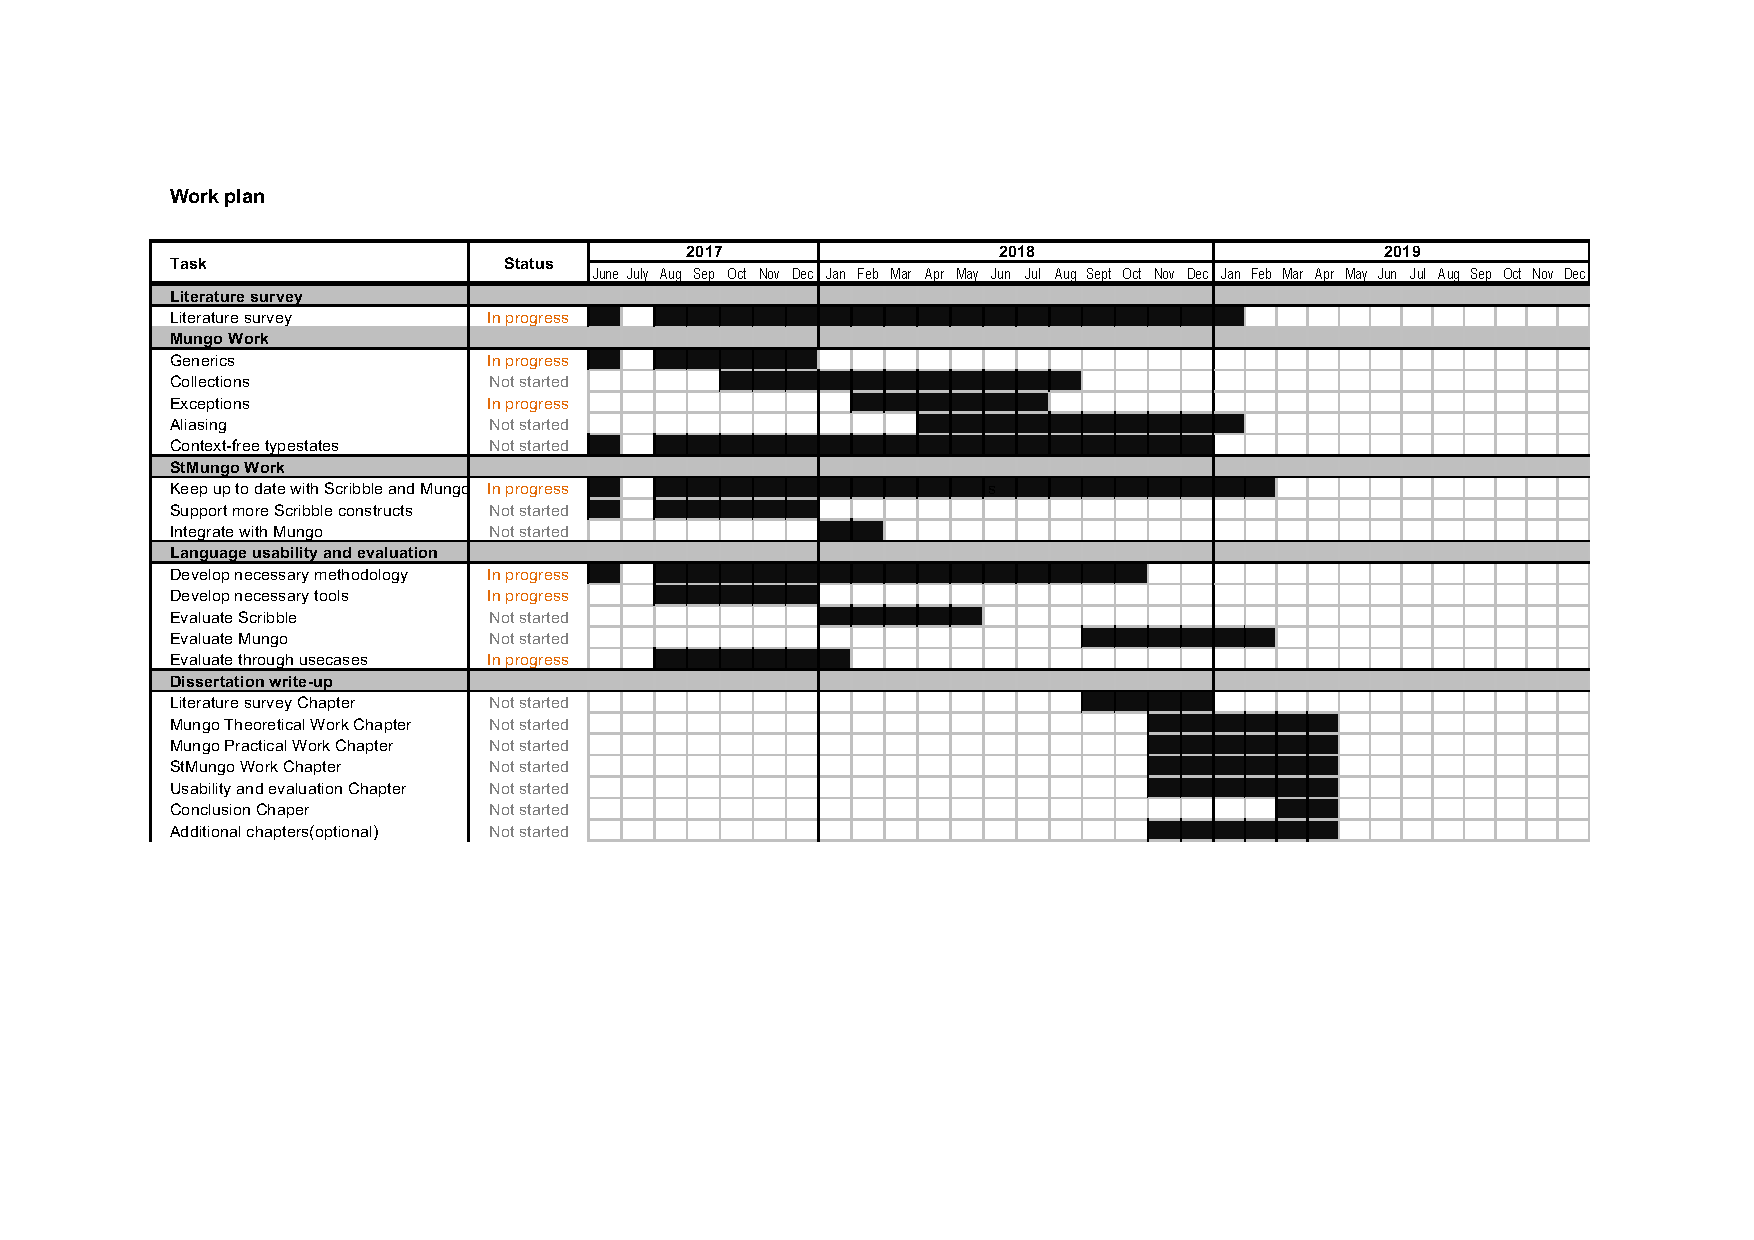
\includegraphics[height=0.9\vsize, width=1.1\hsize]{workplan.pdf}
% \end{figure}
%----------------------------------------------------------------------------------------
% \section{User Study Plan}
% \label{appendix:usertrial}

%----------------------------------------------------------------------------------------
% \section{Training Needs Analysis Form}
% \label{traininglog}
% 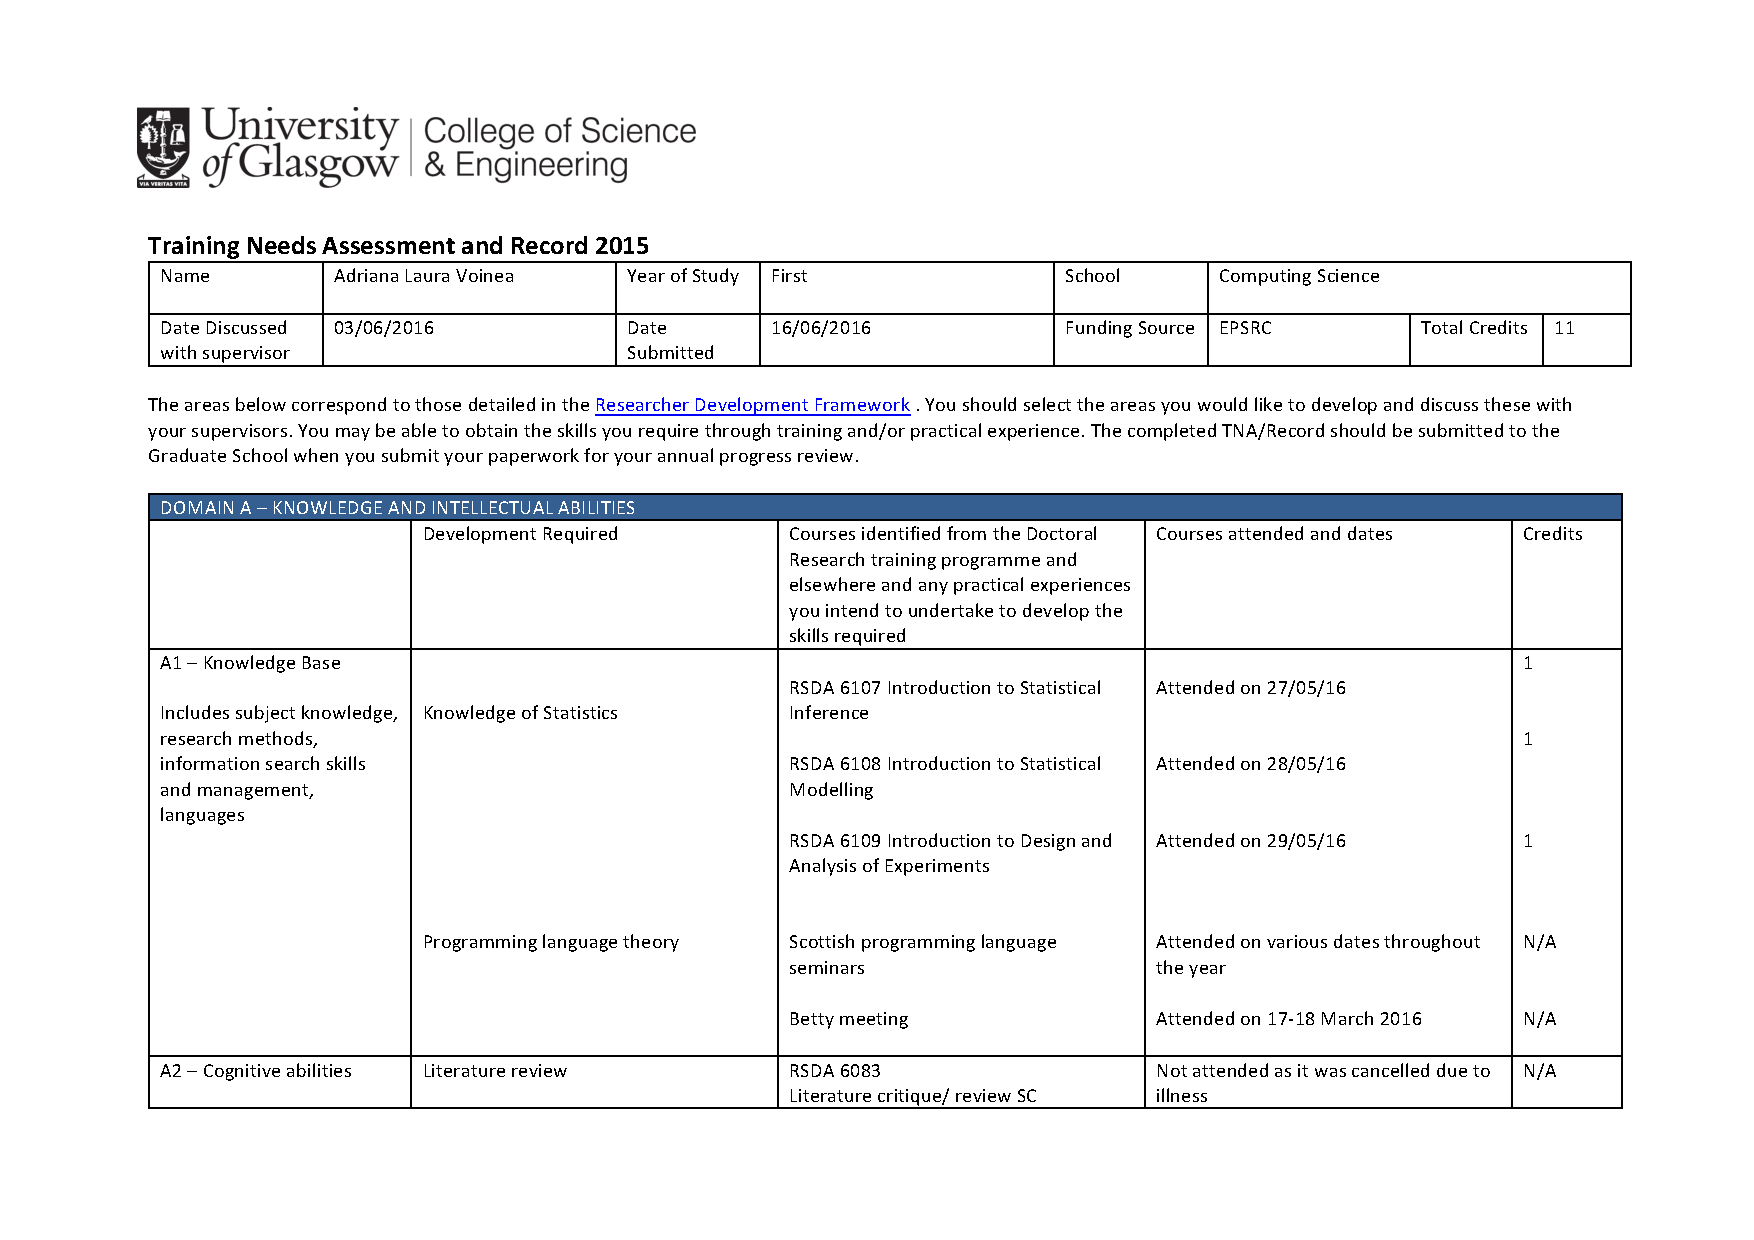
\includepdf[pages=-,landscape=true]{traininglog.pdf}
% %\includepdf[pages=-,pagecommand=\thispagestyle{plain}]{include/form.pdf}

%	BIBLIOGRAPHY
%----------------------------------------------------------------------------------------

\newpage
\bibliographystyle{plain}
\bibliography{report}


\end{document}
